\documentclass{article}
\usepackage[utf8]{inputenc}
\usepackage[spanish]{babel}
\usepackage{listings}
\usepackage{graphicx}
\graphicspath{ {images/} }
\usepackage{cite}

\begin{document}

\begin{titlepage}
    \begin{center}
        \vspace*{1cm}
            
        \Huge
        \textbf{Taller Memoria}
            
        \vspace{0.5cm}
        \LARGE
        Taller - Nociones de la memoria del computador
            
        \vspace{1.5cm}
            
        \textbf{Johan David Rojas Martinez}
            
        \vfill
            
        \vspace{0.8cm}
       
        \Large
\begin{figure}[h]

\includegraphics[width=4cm]{logoudea.png}
\centering
\end{figure}

        \vfill
        Despartamento de Ingeniería Electrónica y Telecomunicaciones\\
        Universidad de Antioquia\\
        Medellín\\
        Septiembre de 2020
                 
    \end{center}
\end{titlepage}

\tableofcontents

\section{Introduccion}
\noindent
Mediante este documento se estará realizando respuesta a algunas preguntas acerca del funcionamiento de la memoria,veremos en general cual es la definición de memoria de un computador, mencionaré los tipos de memoria que conozco y lo que conocía de estas antes de investigar, se mostraran algunas imágenes para ilustrarnos mejor de lo que estamos hablando,también estaremos hablando acerca de cómo es la manera en que se gestiona una memoria y que hace que unas memorias sean más rápidas que otras. 

\section{Preguntas} \label{contenido}

\subsection{Defina qué es la memoria del computador.}
\noindent
La memoria del computador es un dispositivo muy importante para llevar a cabo el correcto funcionamiento de este y según lo entendido sin la memoria nuestro ordenador ni siquiera podría arrancar, la memoria tiene la capacidad de retener, almacenar y memorizar datos, en este dispositivo se almacena temporalmente la informacion que más tarde será utilizada por el microprocesador, esa información realiza un proceso muy particular en nuestra computadora, ya que primero es almacenada en un dispositivo que tiene una alta capacidad de almacenamiento, pero que es más lento que otros dispositvos(ejemplo el disco duro), luego se toma una porción de esta información y es ubicada temporalmente en la memoria RAM(como se habia dicho anteriormente) donde se almacena para poder manipularla posteriormente,más tarde se extraen los datos que se encuentran en la memoria RAM para que el microporocesador haga su trabajo, como ejecutar una serie de instrucciones, calculos necesarios o alguna orden que se le envie,después esa informacion que ya ha sido manipulada o tratada(vulgarmente) se envia a otro lugar de la memoria donde se ubican los documentos ya procesados, este proceso se repite varias veces con todos los documentos que se encuentran apilados en en la memoria a una velocidad demasiado rapida que el humano nunca percibiria, finalemnte cuando ya no hay mas nada que procesar esos docuementos se regresan al disco duro y se eliminan de la memoria RAM para que no ocupen un espacio inecesario. 

\vspace{0.5cm}
\noindent
Este dispositivo es interconectado a la unidad central de procesamiento (CPU, por las siglas en inglés de Central Processing Unit) y los dispositivos de entrada/salida, implementan lo fundamental del modelo de computadora de la \textbf{arquitectura de Von Neumann.}\cite{geniolandia}

\vspace{0.5cm}
\noindent
La memoria se divide en un gran número de piezas pequeñas llamadas celdas. Cada ubicacion o celda tiene una dirección única que varia desde cero hasta el tamaño de la memoria menos uno. por ejemplo, si el ordenador tiene 64 k palabras, entonces esta unidad de momoria tiene 64*1024=65536 posiciones de memoria. La dirección de estos lugares varia de 0 a 65535. \cite{tutorialspoint}


\subsection{Mencione los tipos de memoria que conoce y haga una pequeña descripción de cada tipo.}
\noindent
Los tipos de memoria que conozco y los que he escuchado desde el momento que empecé a manipular computadores y otros dispositivos electrónicos son: memoria RAM, disco duro y memoria caché.
\subsubsection{Memoria RAM}
\noindent
Antes de haber investigado y leer el informe que había sido enviado por el profesor mi idea acerca de la memoria RAM es que era un dispositivo que iba colocado en la placa madre(mother board) del computador y se encargaba de permitirnos abrir varios programas o pestañas en nuestro computador, teniendo tambien la idea de que entre más memoria RAM tuviera nuestro ordenador iba a ser muchisimo más rápido, pues mi idea era que la memoria RAM era la encargada de la velocidad de nuestro PC.

\vspace{0.5cm}
\noindent
Tras haber investigado y leido el material, ya me hago una idea más clara de lo que es la memoria RAM y básicamente es como un escritorio donde ubicamos una información temporalmente que después será utilizada por el microprocesador y se ubica en un espacio de memoria con una direccion exclusiva, entonces tal vez mi idea de que a más memoria RAM más veloz era el computador no era del todo erronea, ya que si por ejemplo contamos con un escritorio bastante amplio(Memoria RAM), se pueden realizar las tareas con más comodidad y podemos almacenar mucha más información sin enredos y con suficiente espacio(es una analogia que puede servir para entender cómo funciona). La memoria RAM almacena la informacion en binarios(1 y 0) suele ser más rapida que otros dispositivos de memoria porque se puede acceder a su información de una forma más rápida y no tan compleja esto se debe a que la informacion es guardada de forma aleatoria,un dato que encontré mientras investigaba por internet y me parecio bastante curioso fue que la memoria RAM es capaz de almacenar datos con tiempos de acceso que oscilan entre 5 a 12 nanosegundos. \cite{geniolandia}

\subsubsection{Disco duro}
\noindent
Lo que entendía por disco duro es que este es un dispositivo electrónico y que parte de su funcionamiento es de forma mecánica, se encuentra ubicado dentro de la torre del ordenador, donde se almacena la información de nuestro sistema, nuestros archivos tambien se encuentran aquí de forma permanente, incluso aunque apaguemos nuestro PC.
Los discos duros los podemos encontrar en el mercado con distintas capacidades de almacenamiento, por ejemplo: 250GB, 500GB, 1TB,etc,entre más capapacidad tenga nuestro disco duro más información y archivos podremos tener en nuestra computadora y es en este mismo donde tenemos instalado nuestro sistema operativo que es el que nos permite interactuar con la máquina y con los dispositivos periféricos de una forma más dinamica. El disco duro suele ser uno de los dispositivos más lento que tiene nuestro computador pero a su vez uno de los más amplios en memoria. 

\vspace{0.2cm}
\noindent
El principal funcionamiento de un disco duro se basa en que los cabezales pongan marcas magnéticas en las pistas del plato con 3 posiciones diferentes estas pueden ser: 1, 0 ó neutro y las máquinas son capaces de decodificar ese código binario como información. Al momento de guardar un archivo en el disco duro de nuestro PC, este escribe en los platos una secuencia de unos y ceros a velocidades que se miden en micro segundos. \cite{qloudea}
\vspace{0.2cm}
\noindent
\emph{A continuacion se muestra una imagen de como es físicamente un disco duro}(\ref{fig:disco_duro})

\begin{figure}[h]
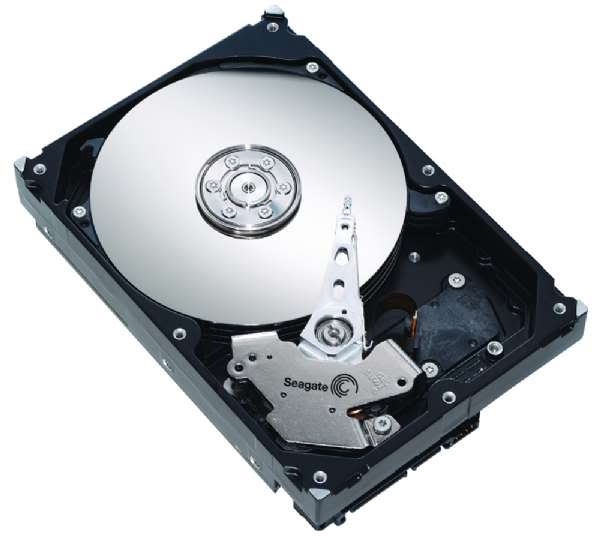
\includegraphics[width=6cm]{disco_duro.jpg}
\centering
\caption{Imagen del disco duro}
\label{fig:disco_duro}
\end{figure}

\subsubsection{Memoria caché}
\noindent
La memoria caché segun lo que entendí de la definicion del documento que nos envio el profesor Augusto \cite{Augusto} es que esta se utiliza para trabajar con la información que el microprocesador nota que es utilizada de forma muy seguida, entonces para este no tener que buscarla de nuevo y ejecutar siempre esas mismas instrucciones la guarda en la memoria caché y puede reutilizarla cuantas veces quiera, esta memoria es mucho más rápida que las mencionadas anteriormente, pero a su vez tiene un alto costo y cuentan con poca capacidad de almacenamiento(12 megabytes normalmente).

\vspace{0.3cm}
\noindent
Los computadores modernos han venido incorporando esta nueva tecnologia en tres niveles(L1 ,L2,L3), la memoria L1 se encuentra incorporada dentro de los núcleos del microprocesador y es una de las más rápidas, pero con menos capacidad de almacenamiento esta se divide en dos partes una para datos y otra para instrucciones cada una cuenta con 32 kilobytes, la memoria caché L2 hoy en dia los fabricantes también la incorporan dentro de los núcleos del microprocesador en comparación con la L1 es un poco más lenta,pero con más almacenamiento, ya que cuenta con 256 kilobytes de capacidad para almacenar datos e instrucciones, finalmente la memoria caché L3 se encuentra incorporada dentro del procesador pero fuera de los núcleos y es la más lenta de todas (sin dejar de ser más rapida que la memoria RAM que se encuentra instalada en la \textbf{motherboard}), esta es la que cuenta con más capacidad de las 3 memorias caché contando con una capacidad de 12 MB. 

\subsection{Describa la manera como se gestiona la memoria en un computador.}
\noindent
Para que un programa pueda ser ejecutado correctamente en un computador es necesario principalmente cargarlo en la memoria; mientras este se  ejecuta, el programa accede a sus instrucciones o datos que se encuentran ubicados en la memoria, posteriormente el programa termina su proceso de ejecucion y el espacio de memoria que estaba siendo utilizado para acceder a sus instrucciones o datos se declara como disponible, y el siguiente programa puede cargarse y ejecutarse, este proceso se realiza tantas veces como iniciemos y terminemos el proceso de ejecución de un programa.

\noindent
La principal funcion del sistema operativo en la gestion de la memoria es:
\begin{itemize}
\item Saber cuáles son las partes de la memoria que se están usando actualmente y qué las está usando.
\item Decidir qué procesos se cargarán en la memoria cuando haya algun espacio disponible.
\item Asignar y liberar espacio de memoria según se necesite.
\item La Memoria Principal es un recurso muy importante que se debe gestionar, ya que necesitamos velocidad al ejecutar un programa.
\cite{sites.google}

\end{itemize}

\subsection{¿Qué hace que una memoria sea más rápida que otra? ¿Por qué esto es importante?}
\noindent
Lo que hace que una memoria sea más rápida que otra es su latencia, esta es la eficiencia que puede tener un módulo de memoria, la latencia esta vinculada en una gran medida con un proceso muy particular que es la lectura y la escritura de los datos o información que se encuentre almacenada en la memoria.

\vspace{0.3cm}
\noindent
La latencia es basicamente la cantidad de tiempo que transcurre desde que el controlador de memoria recibe la orden del microprocesador de recoger alguna serie de datos y estos son obtenidos, Por lo tanto cuanto menor sea ese tiempo de espera entre peticiones, más eficiente es la memoria y más fluidez aportará al sistema. \cite{computerhoy}. 
si estudiamos el nivel de latencia de una memoria tambien es muy importante estudiar su frecuencia.

\vspace{0.3cm}
\noindent
La \textbf{frecuencia} viene dada en unidades de Megahercios (MHz), ese valor nos indica la velocidad a la trabajan los chips de memoria integradas en cada módulo. entonces, a mayor cantidad de Megahercios, mayor velocidad tendrá el módulo de memoria. Por otro lado, la frecuencia nos define la velocidad a la que se transportan los datos de lectura y escritura. 


\vspace{0.3cm}
\noindent
Existe una fórmula matemática sencilla para calcular, de forma aproximada, el rendimiento que tendrían los módulos de memoria RAM en nanosegundos, a pesar de tener diferentes parámetros de frecuencia y latencia.\cite{computerhoy}

La fórmula sería algo así: (\ref{fig:formula})
\begin{figure}[h]
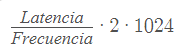
\includegraphics[width=6cm]{formula.PNG}
\centering
\caption{formula}
\label{fig:formula}
\end{figure}

\noindent
Finalmente, hay otro factor que tambien puede tener una alta influencia al analizar porque una memoria es más rapida que otra y esto se debe a que algunas memorias por ejemplo; la memoria DRAM por cada celda tienen un transistor y un capacitor(por lo tanto una memoria de este tipo tiene millones de transistores y capacitores y nos permite tener más capacidad de almacenamiento que otras memorias), los capacitores deben mantener llenandose de electrones los cuales representan información(Esto ocurre en milisegundos) y para mantener los capacitores con la misma información (1 y 0) el controlador de la memoria debe mantenerse llenandolos constantemente con 1, ese proceso de recarga se realiza muchas veces por segundos, pero ya en otros tipos de memorias como por ejemplo: La memoria estática (SRAM) utiliza una tecnologia diferente(en esta cada celda de bit está compuesta por cuatro o seis transistores y algunos circuitos,lo que implica que su capacidad de almacenamiento se reduzca mas que en otras pero no su rapidez), debido a esto no es necesario recargar las celdas constantemente para mantener la información, como sucede con la memoria dinámica. El ejemplo anterior nos muestra como este factor puede permitir que una memoria sea más rapida que otra(esto mismo hace que la memoria SRAM sea más rápida y tenga menos capacidad que la DRAM).\cite{Augusto}

\vspace{0.3cm}
\noindent
\textbf{¿Por qúe esto es importante?}

\vspace{}
\noindent
El hecho de que una memoria sea rapida es muy importante ya que esto nos define en cierta medida la velocidad a la que se van a transportar los datos de lectura y escritura. se podría pensar que entre más rápida sea la memoria de nuestro ordenador, más influirá en el rendimiento de este mismo, ya que podrá ser capaz de resolver una mayor cantidad de operaciones e instrucciones por segundo.
\noindent
Lo anterior no significa que solo por tener una memoria bastante rápida y con alta frecuencia ya es suficiente, pero si es un punto muy importante si queremos conseguir un mejor rendimiendo por parte de nuestra computadora. \cite{computerhoy}

\section{Conclusión} \label{conclulsion}
\noindent
Tras realizar este taller pudé aprender que un computador es una herramienta altamente veloz que se compone de dispositivos electrónicos interconectados entre sí, llevandolo a ser una invención bastantemente compleja, pero a su vez reducido a una arquitectura simple(sin dejar de ser muy potente) y en la que todos los computadores y aparatos electrónicos se encuentran basados en la actualidad, estos utilizan  lo que se conoce como la arquitectura de John Von Neumann, además que todos nuestros sistemas de cómputo están compuestos por una memoria y se acompaña de un microprocesador el cual le permite realizar sus tareas de una forma más veloz e inteligente, además que existen distintos tipos de memorias que pueden variar en velocidad, almacenamiento y costos.

\bibliographystyle{IEEEtran}
\bibliography{references}

\end{document}
